
%\documentclass[british, journal]{IEEEtran}
\documentclass[british,conference,compsoc]{IEEEtran}
\usepackage[T1]{fontenc}
%\usepackage[latin9]{inputenc}
\usepackage{float}
\usepackage{amsmath}
\usepackage{amssymb}
\usepackage{graphicx}
\usepackage{setspace}
\usepackage{array}
\usepackage{blindtext}

\makeatletter

\newcommand{\noun}[1]{\textsc{#1}}

\@ifundefined{showcaptionsetup}{}{
 \PassOptionsToPackage{caption=false}{subfig}}
\usepackage{subfig}
\makeatother

\usepackage{babel}
\usepackage{algpseudocode}
\usepackage{algorithm}

\begin{document}

\twocolumn

\title{Automated translation of asynchronous concepts \\
to Signal Transition Graphs}
\author{Jonathan Beaumont\\
\texttt{j.r.beaumont@ncl.ac.uk}\\
\emph{School of Electrical and Electronic Engineering, Newcastle University,
UK}}

\maketitle

\begin{abstract}
Asynchronous circuits are becoming increasingly important in
system design for Internet-of-Things, where they orchestrate
the interface between big synchronous computation components
and the analogue environment, which is inherently asynchronous
and has high uncertainty with respect to power supply,
temperature and long-term ageing effects.
However, wide adoption of asynchronous circuits by industrial users is
hindered by a steep learning curve for asynchronous control models,
such as Signal Transition Graphs, that are developed by the academic
community for specification, verification and synthesis of
asynchronous circuits.

Previously, we have introduced a novel high-level description language
for asynchronous circuits, which is based on behavioural
\textit{concepts} -- high-level descriptions of asynchronous circuit
requirements, that can be shared, reused and extended by users. 
In this paper we will discuss more examples using concepts, and an algorithm to
automatically translate these to Signal Transition Graphs for further processing
by conventional asynchronous and synchronous EDA tools, such as \noun{Petrify}
and \noun{Mpsat}. Our aim is to simplify the process of capturing system
requirements in the form of a formal specification, and to promote behavioural
concepts as a means for design reuse. The proposed design flow is fully
automated in open-source toolsuite \noun{Workcraft}.
\end{abstract}

\sloppy
\thispagestyle{empty}
%%\vspace{-3mm}
\section{Introduction}

\emph{Concepts} have been presented in order to provide a more compact, adaptive and intuitive method of
designing asynchronous circuits, using a fully compositional text based description method. 
This was born out of the use of algebra for designing systems,
such as the model Conditional Partial Order Graphs~\cite{CPOG1}\cite{CPOG2}\cite{2014_mokhov_pg},
the algebra of switching networks~\cite{mokhov2015algebra}. Composition is an important part of concepts
 and the use of composition in some algebraic representations, such as with DI algebra~\cite{270632} 
 and Conditional Signal Graphs~\cite{6243877} helped to inspire this. 

As discussed in~\cite{2015_Beaumont_MEMOCODE}, concepts are a useful language for specifying
the behaviours of asynchronous circuits, in the preferred form of the user. This can be as low-level 
signal-level concepts, or higher-level gate- or protocol-level concepts. It also allows the definition of 
their own concepts, which can be reused within the same or any other specification that they wish
to increase the speed of designing a system, and future systems. 

With concepts, we aim to solve the problems that can arise from the more commonly used
monolithic approach, where a user must design each system in the form of an STG from a blank page. 
The scalability of this is poor: as the system grows in complexity its monolithic specification becomes 
challenging to comprehend and debug. The problem becomes particularly severe when designing 
multi-mode systems, such as power regulators, where capturing all aspects of system behaviour in a
consistent specification is a major design challenge~\cite{2014_sokolov_ftfc}\cite{sokolov2015design}. 
Moreover, the STG models of components and  operating modes are difficult to reuse when designing 
other specifications, and thus each new design must be built from the ground up. This is particularly 
undesirable for industry, as this increases the design time of each design greatly. 

STGs~\cite{Chu_1987_phd}\cite{Rosenblum_1985_tpn}
are commonly used for the specification,
verification and synthesis of asynchronous control circuits as they are
supported by multiple EDA tools, such as \noun{Petrify}~\cite{Cortadella},
\noun{Mpsat}~\cite{khomenko2004detecting}, \noun{Versify}~\cite{i1997formal},
\noun{Workcraft}~\cite{2007_poliakov_workcraft}\cite{Workcraft_website}, and
others.
These tools take an STG specification of a complete controller and can
formally verify its correctness, as well as synthesise an asynchronous
circuit implementation that is \emph{speed-independent}, i.e. guaranteed
to work correctly regardless of component delays~\cite{Muller_1959_ts}.

Concepts are not supported by these tools, and rather than reinvent the wheel by authoring tools
to verify and synthesize concepts directly, we can \emph{translate} concepts to STGs, for use with 
these existing tools. Previously, we have introduced a prototype algorithm for translating concepts
to STGs. However, this version would not allow for some important features of circuits to be
translated. 

In this paper we display all concept types necessary for a complete specification, and some 
example concept specifications. These will display the possibilities of concepts, as well as the 
problems with the prototype translation algorithm, namely \emph{OR-causality}, which is 
much more complex than AND-causality which is standard within concepts. 
This will lead us to a new translation algorithm, which has been implemented as a tool. 
%along with the domain specific language~\cite{2016_concepts_github} embedded in 
%Haskell~\cite{1996_hudak_dsl}, and integrated into 
%\noun{Workcraft}~\cite{Workcraft_website}, an open-source EDA tool which also 
%features some verification and synthesis tools for STGs. 

Our contributions are as follows:
\begin{itemize}
  \item We detail the concepts required for a successful  
  translation in Section~\ref{sec:trans-concepts}
  \item We introduce some new gate examples and their specifications in
  Section~\ref{sec:examples}, presenting what can be acheived with
  concepts, and how OR-causality becomes necessary in specifications.
  \item We present the implemented algorithm for translating concepts to STGs
  including OR-causality in Section~\ref{sec:algorithm}.
\end{itemize}

\noindent
We start with a brief recap of asynchronous concepts as a specification language in
Section~\ref{sec:async-concepts}, and discuss the interoperability of the provided tool 
with existing standard STG based tools in Section~\ref{sub:interop-with-stg}.

%\vspace{-3mm}

\section{Asynchronous Concepts\label{sec:async-concepts}}

%\vspace{-2mm}

The abstract base of the concepts, on which these asynchronous specific circuits
is discussed in~\cite{2015_Beaumont_MEMOCODE}.

\textbf{\label{signal-level}Signal-level concepts:} Asynchronous circuit specifications
are mainly composed of signal transitions, and interactions between these, to show
causal relationships. Signal transitions are denoted as $a^{+}$ and $a^{-}$, where $a$ is
any signal name, at least one character, and the $+$ or $-$ indicates which way the 
this signal transitions, $+$ denoting a low-to-high or 0 to 1 transition, and $-$ denoting
a high-to-low, 1 to 0 transition. 

Signal-level concepts are the base level of concepts, and are 
the type all other concepts are built on. Here we display the standard concepts
available at this level.

A key concept in asynchronous circuits is \emph{causality}:
one signal transition \emph{causes} another signal transition, a cause and an effect.
This is denoted in the form: 
\[
a^{+}\rightsquigarrow c^{+}
\]
This is read as $a^{+}$ causes $c^{+}$, meaning that for the $c^{+}$ transition to
occur, $a^{+}$ must have occurred previously. The $\rightsquigarrow$ operator is
used to show causal relationships between signals.
 
While this concept is called \emph{causality}, this doesn't necessarily imply
timings, such as any $\mathit{cause}$ transition immediately forcing the
 $\mathit{effect}$ transition it applies to. Causality can be used in order to
list all possible $\mathit{cause}$ transitions which need to occur in order
 for an $\mathit{effect}$ transition.

One can compose any concepts using the $\diamond$ (diamond) operator, and this applies
to concepts of any level, whether predefined or user-defined. For example, 
two causality concepts can be composed.
\[
a^{+}\rightsquigarrow c^{+}\ \diamond\ b^{+}\rightsquigarrow c^{+}
\]
In words, $a^{+}$ \emph{and} $b^{+}$ must occur before $c^{+}$ can occur. 
This corresponds to so-called AND-causality in the fact that several cause transitions \emph{must all}
have occurred before an event can occur. AND-causality is commonly used
to imply behaviours in circuits, for specific requirements of effect transitions.  

The above notation can cause long-winded specifications when lots of AND-causality is involved. 
To solve this we provise a listing option. The following will acheive the same results:

%\vspace{-3mm}

\[
[a^{+}, b^{+}]\sim\hspace{-1.5mm}\&\hspace{-1.5mm}\sim\hspace{-1.5mm}>c^{+}
\]
This form of concept can be composed as usual with any other concepts.

A less common, but still useful form of causality is OR-causality. This is where an effect transition
can have several possible cause transitions. Only one cause transition is required to occur to allow
the effect transition to occur. 

With OR-causality, the notation used lists all possible causes for the stated effect:

%\vspace{-3mm}

\[
[x^{+}, y^{+}]\sim\hspace{-1.5mm}|\hspace{-1.5mm}\sim\hspace{-1.5mm}>z^{+}
\]

This is, \emph{either} $x^{+}$ \emph{or} $y^{+}$ must occur in order for 
$z^{+}$ to occur.

The interactions when an effect transition is included in both AND- and OR-causality are interesting, and
an example of when this occurs can be found in Section~\ref{sec:algorithm}, along with a description
of the implemented algorithm, which discusses the issues OR-causality poses with translation.

\textbf{Gate-level concepts:} Using the causality concept we can express
the behaviour of gates in asynchronous circuits. For example, a \emph{buffer}
is a gate with one input signal and one output signal ,
whose output transitions causally depend on the input ones:
\[
\mathsf{buffer}(a, b)=a^{+}\rightsquigarrow b^{+}\ \diamond\
a^{-}\rightsquigarrow b^{-}
\]

\noindent An \emph{inverter} has a similar conceptual specification, but the
output transition is inverted:
\[
\mathsf{inverter}(a, b)=a^{+}\rightsquigarrow b^{-}\ \diamond\
a^{-}\rightsquigarrow b^{+}
\]

\noindent A \emph{C-element} is a gate with two inputs, in this example $a$ and $b$ and one
output~$c$, which synchronises both rising and falling input transitions
via AND-causality:
\[
\mathsf{cElement}(a, b, c)=a^{+}\!\rightsquigarrow\! c^{+}\ \diamond\
b^{+}\!\rightsquigarrow\! c^{+}\ \diamond\ a^{-}\!\rightsquigarrow\! c^{-}\
\diamond\ b^{-}\!\rightsquigarrow\! c^{-}
\]

An alternative way to express the same concept is to reuse the buffer concept:
\[
\mathsf{cElement}(a, b, c)=\mathsf{buffer}(a, c) \diamond \mathsf{buffer}(b, c)
\]
A C-element combines the constraints imposed on the output
transitions by two `virtual' buffers. An expanded example of a C-element can be
found in~\cite{2015_Beaumont_MEMOCODE}.

Behaviour of other gates can be similarly defined using concepts. We will dicuss
this in Section~\ref{sec:examples}.

\textbf{Protocol-level concepts:} In addition to gate-level concepts
described above it is often important to specify \emph{protocols}
of interaction between multiple gates, components or signals. 

Here we demonstrate how one can use concepts to specify asynchronous handshakes
and mutual exclusion mechanisms.

Given two signals $a$ and $b$, a \emph{handshake} between them is
the following composition of causality concepts:
\[
\mathsf{handshake}(a, b)=a^{+}\!\rightsquigarrow\! b^{+}\ \diamond\
b^{+}\!\rightsquigarrow\! a^{-}\ \diamond\ a^{-}\!\rightsquigarrow\! b^{-}\
\diamond\ b^{-}\ \rightsquigarrow\! a^{+}
\]
Intuitively, we have a two-way asynchronous communication channel,
where one party sends transitions $a^{+}$ and $a^{-}$ and the other
party responds by corresponding $b^{+}$ and $b^{-}$ transitions.
Note that the four causality concepts match those found
in the buffer and inverter concepts, which leads to an alternative
way to express a handshake between~$a$ and~$b$:
\[
\mathsf{handshake}(a, b)=\mathsf{buffer}(a, b) \diamond\mathsf{inverter}(b, a)
\]
This conceptual understanding of a handshake as being composed
from a buffer and an inverter is often used by circuit designers as
a convenient way of reasoning.

The last standard concept is \emph{mutual
exclusion} between two signals~$a$ and~$b$:
\[
\mathsf{me}(a, b) = a^{-}\rightsquigarrow b^{+}\ \diamond\ b^{-}\rightsquigarrow
a^{+}
\]
The concept states that, in terms of causality, rising transitions 
$a^{+}$ and $b^{+}$ can only occur after
the opposite falling signal transitions. Therefore, even if all other cause-transitions for
either $a^{+}$ or $b^{+}$ have occurred, while the one signal is high, this blocks 
the other from transitioning high. This guarantees that $a$ and
$b$ are never set to $1$ at the same time, i.e. they are mutually
exclusive.

We can now specify a \emph{mutual exclusion
element}~\cite{2008_kinniment_synchronisation}
that receives asynchronous requests $r_{1}$ and $r_{2}$ to a shared
resource and grants access to it by corresponding mutually exclusive
signals $g_{1}$ and $g_{2}$:

%\vspace{-3mm}
{\small
\[
\mathsf{meElement}(r_{1}, r_{2}, g_{1}, g_{2})\!=\!\mathsf{buffer}(r_{1}, g_{1})
\diamond \mathsf{buffer}(r_{2}, g_{2}) \diamond \mathsf{me}(g_{1}, g_{2})
\]}

%\vspace{-8mm}

\section{Concepts for translation\label{sec:trans-concepts}}

The concepts we have discussed so far are aimed at specifying the behaviour of signals in a circuit.
When translating these to STGs however, these behaviours do not necessarily result in a correct
specification, meaning they will not be verifiable by standard tools, and therefore not useful in 
further operations, such as synthesis.

This is due to various parts of an STG that we have not yet discussed, which are important
for specification, namely \emph{interface} and \emph{initial states}.

%\vspace{-5mm}

\subsection{Interface concepts \label{sub:interface}} 

An important part of a specification is how these signals interact with the outside world, which could
be another scenario or another circuit, for example. These signals can be inputs from the outside world,
outputs or an internal signal, which is used only within this scenario. 

To specify the type of a signal (\emph{input},
\emph{output} or \emph{internal}) we introduce the \textsf{interface} concept:
\[
\mathsf{interface} : A \rightarrow \{\mathsf{Input}, \mathsf{Output},
\mathsf{Internal}\}
\]
Signal types are composed according to the following rules:
\[
\begin{array}{|l||l|l|l|}
\hline
\multicolumn{1}{|c||}{\diamond} & \mathsf{Input} & \mathsf{Output} &
\mathsf{Internal} \\ \hline \hline
\mathsf{Input} & \mathsf{Input} & \mathsf{Output} & \mathsf{Internal} \\ \hline
\mathsf{Output} & \mathsf{Output} & \mathsf{Output} & \mathsf{Internal} \\
\hline
\mathsf{Internal}& \mathsf{Internal} & \mathsf{Internal} & \mathsf{Internal} \\
\hline
\end{array}
\]
The intuition is as follows:
\begin{itemize}
    \item If a signal is an input in one component of the system, but is an
    output in another components, then in the composition it will be an output.
    \item An internal signal is similar to an output signal in the sense
that it is driven by the circuit (not the environment), but it is hidden, i.e.not accessible via the circuit interface. Once a signal is hidden and declared    internal it cannot be revealed.
\end{itemize}

\noindent Specifying signal types is important when designing asynchronous
circuits, as it helps to quickly identify errors (e.g. an input transition is
caused by a hidden internal transition), and reuse existing tools for circuit
simulation, verification and synthesis. Signal type information is also used
in the algorithm for automated translation of concepts to
STGs (Section~\ref{sec:algorithm}).

Concepts \textsf{inputs}, \textsf{outputs}, \textsf{internals} are defined for
specifying types of sets of signals for convenience, and to be included inline with other
concepts. For example, to specify
that signals $a$ and $b$ are inputs, $c$ is an output, and $t$ is internal, it
is possible to write:
\[
\mathsf{inputs}(\{a, b\}) \diamond \mathsf{outputs}(\{c\}) \diamond
\mathsf{internals}(\{t\}).
\]

%\vspace{-5mm}

\subsection{Initial state concepts \label{sub:initState}}

Specifying the initial state is important, as it determines what the first transitions
of a scenario will be. Without these, no transition can occur.

Each signal must have it's initial state declared before translation can occur. 
In order to specify the initial state of a handshake between signals~$a$
and~$b$, we use the $\mathsf{initialise}$ concept:
\[
\mathsf{initialise}(\mathit{signal},\mathit{value})=\mathsf{after}(signal,
value)
\]

\noindent The possible initial states are \emph{high} or \emph{low}, referred to as \emph{0} 
or \emph{1} respectively:

\[
\mathsf{initialise}(a,0) \diamond \mathsf{initialise}(x, 1)
\]

\noindent A signal can only be declared as initially high or low. If the initial state of a signal is 
not defined, and error will occur, and the translation will not continue. Conversely, 
if the event a signal has it's initial state declared as both high and low,
and is thus inconsistent, in a specification then the translation will also fail.

For the ease of use, and to speed up the process, initial states can also be declared
in lists by on state:

\[
\mathsf{initialise0} [a, b, c] \diamond \mathsf{initialise1} [x, y]
\]


\noindent As an example, we can include this in the specification of a handshake, to 
create a handshake with built-in initial state.
$\mathsf{initialise}(a, 0)$ sets the state of the signal
$a$ to $0$. We can compose an initial state concept with the handshake concept
into a combined $\mathsf{handshake00}(a, b)$ concept as
\[
\mathsf{handshake00} = \mathsf{handshake}(a, b) \diamond \mathsf{initialise}(a, 0) \diamond
\mathsf{initialise}(b, 0)
\]
The resulting concept corresponds to a handshake between signals~$a$
and~$b$ that are both initially $0$.

%\vspace{-3mm}

\section{Concept examples \label{sec:examples}}

In our previous paper, \cite{2015_Beaumont_MEMOCODE}, we have 
used a C-element as a small example of how we can specify a standard gate with concepts,
and how there are several ways of describing these with concepts. 

In this section, we will discuss the concept specification of some different gates,
a Set-Reset latch which uses AND-causality, and an OR-gate and an AND-gate, both of 
which use both AND- and OR-causality, and this proves to be more difficult to translate,
which we will use an example in Section~\label{translation-algorithm}.

%\vspace{-3mm}

\subsection{Set-reset latch \label{sub:srlatch}}

A set-reset latch (S-R latch) is a particularly simple logic gate, used to store either a zero or one,
depending on the inputs. 

%\vspace{-5mm}

\begin{figure}[h]
\begin{centering}
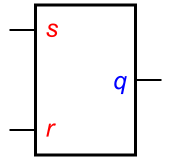
\includegraphics[scale=0.51]{Images/sr-latch-circuit}
\par\end{centering}
%\vspace{-1mm}
\protect\caption{\label{fig:sr-latch-circuit} The symbol of an SR-latch}
%\vspace{-3mm}
\end{figure}

\noindent There are two input signals for this gate, $s$ and $r$, and a single output, $q$: 

\begin{itemize}
  \item $s$: \emph{set} - When this signal is high, it sets the output, meaning it sets it high.
  \item $r$: \emph{reset} - When this signal is high, it resets the output, meaning it sets it low.
  \item $q$: \emph{latched bit} - This stores the desired value, set depending on the values of the input signals.
\end{itemize}

\noindent From this information, we can start to specify the gate with concepts.

First of all, we know the types of these signals, so let us sepcify the interface concept.

%\vspace{-2mm}

\[
\begin{array}{lcl}
\mathsf{interface}&\hspace{-2mm}=&\hspace{-2mm}\mathsf{inputs}[s, r]~\diamond~\mathsf{outputs}[q]
\end{array}
\]

\noindent Now we move onto the interaction between signals. First of all, to set the output high.
When $s$ is high, this causes $q$ to go high. However, only after $s$ goes low can $q$ go low.
In concepts this is: 

%\vspace{-3mm}

\[
\begin{array}{lcl}
\mathsf{set}&\hspace{-2mm}=&\hspace{-2mm}s^{+} \rightsquigarrow q^{+} \diamond\, s^{-} \rightsquigarrow q^{-}
\end{array}
\]

\noindent The interaction between the reset signal and the output will be opposite to this; $r$ going high causes $q$ 
to go low. Only after $r$ goes low can $q$ go low. The concept for this is:

%\vspace{-2mm}
\[
\begin{array}{lcl}
\mathsf{reset}&\hspace{-2mm}=&\hspace{-2mm}r^{+} \rightsquigarrow q^{-} \diamond\, r^{-} \rightsquigarrow q^{+}
\end{array}
\]

\noindent The next concept to specify is the initial state. The description given mentions nothing
to help with the initial state, but let's assume we would like the output to initially be 0. 
To then allow the S-R latch to react only to the inputs, we can set the initial states of the 
inputs to 0 too. This will mean that $s$ is not trying to take the output high, and $q$ is not
blocking the output from going high. 

\[
\begin{array}{lcl}
\mathsf{initialState}&\hspace{-2mm}=&\hspace{-2mm}\mathsf{initialise0} [s, r, q]
\end{array}
\]

\noindent Finally, we can compose all of these concepts, in order to translate them to an STG. This concept will be:

%\vspace{-3mm}

\[
\begin{array}{lcl}
\mathsf{SRLatch}&\hspace{-2mm}=&\hspace{-2mm}\mathsf{set} \diamond\, \mathsf{reset} \diamond\, \mathsf{interface} 
\diamond\, \mathsf{initialState}.
\end{array}
\]

\noindent It is possible reuse some previously defined concepts for the specification of an SRLatch,
which may be preferred by users, as these describe their behaviour in terms of gates.  

The $set$ concept features the same signal-level concepts as a buffer, and thus can be redefined
as a buffer of $s$ and $q$. Similarly, the $reset$ concept can be replaced by an inverter between
$r$ and $q$. Two gates cannot be connected in this way in an actual circuit, however
it defines their behaviours in a different way, which may be understood better in some cases.

Since this now reduces the number of concepts, and thus the length of the specification, we
can define an SR-latch as follows:

%\vspace{-3mm}

 \[
\begin{array}{lcl}
\mathsf{SRLatch}&\hspace{-2mm}=\mathsf{buffer}(s, q) \diamond\, \mathsf{inverter}(r, q) \diamond\, \mathsf{inputs}[s, r]\\ 
&\diamond\, \mathsf{outputs}[q] \diamond\, \mathsf{initialise0} [s, r, q]
\end{array}
\]

\noindent It's isn't necessary to split a scenario specification up into several concepts. 
Depending on the size of the specification, it may be simpler and quicker to 
produce a single concept like this.

Either of these concept specifications can be translated to produce an STG. 
The translated STG can be found in Figure~\ref{fig:sr-latch-stg}.

%\vspace{-3mm}

\begin{figure}[h]
\begin{centering}
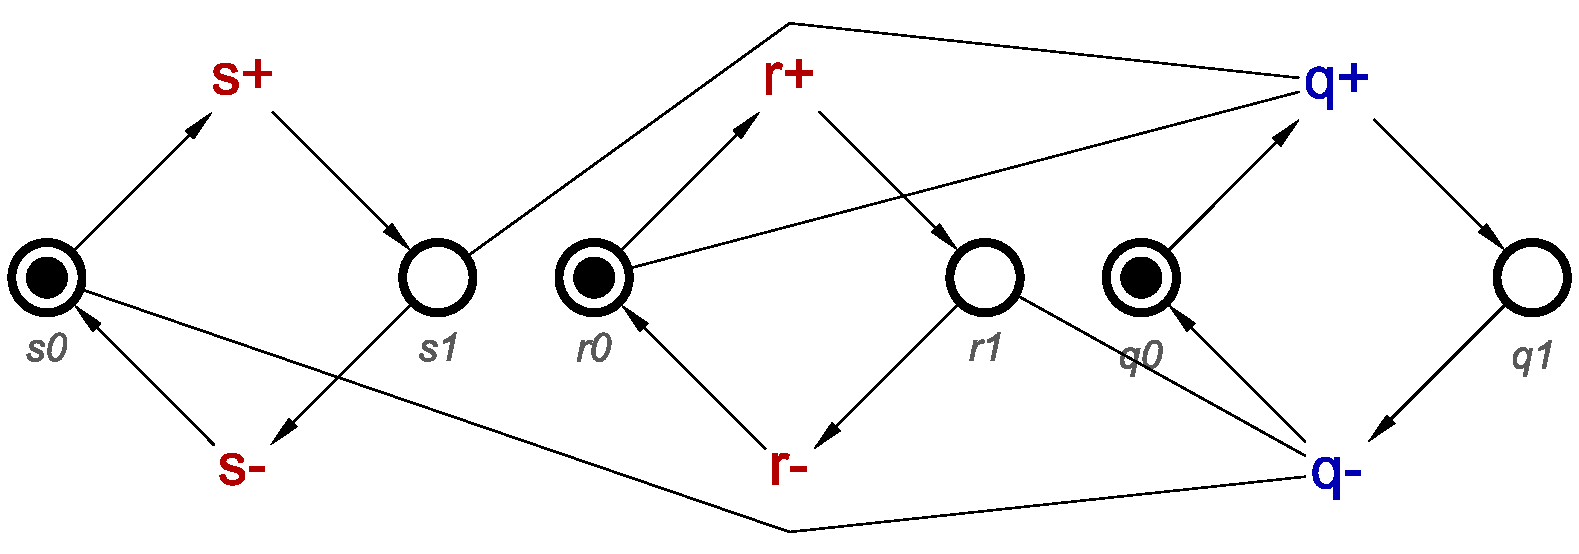
\includegraphics[scale=0.25]{Images/sr-latch-stg}
\par\end{centering}
%\vspace{-1mm}
\protect\caption{\label{fig:sr-latch-stg} An SR-latch STG}
%\vspace{-5mm}
\end{figure}

%\vspace{-5mm}
\subsection{OR-gate \label{sub:or-gate}}

The S-R latch features only AND-causality, and as we displayed 
in~\cite{2015_Beaumont_MEMOCODE}, with the examples of a C-element 
and a Buck controller, which only feature AND-causality, these can be translated
to an STG. 

OR-causality is quite different however, and causes some significant differences 
in a resulting STG, as we will see with the example of an OR-gate. 

\begin{figure}[h]
\begin{centering}
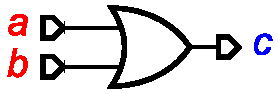
\includegraphics[scale=0.55]{Images/or-gate-circuit}
\par\end{centering}

\protect\caption{\label{fig:or-gate-circuit} The circuit diagram of an OR-gate}
%\vspace{-3mm}
\end{figure}

Let's start by specifying the OR-gate. There are three signals, which for this 
example we will call $a$ and $b$ which are inputs, and $c$ which is the only output:

\begin{itemize}
  \item $a$ - When either this signal or $b$ is high, the output should be set high.
  \item $b$ - When either this signal or $a$ is high, the output should be set high.
  \item $c$ - This output signal is high when at least one of the inputs is high, but low when
		\emph{both} input signals are low.
\end{itemize}

As with the S-R latch, we can start by specifying the interface: 

%\vspace{-4mm}

\[
\begin{array}{lcl}
\mathsf{interface}&\hspace{-2mm}=&\hspace{-2mm}\mathsf{inputs}[a, b]~\diamond~\mathsf{outputs}[c]
\end{array}
\]

\noindent Again, there is no information on the initial state. By the description, we can
assume that setting all signals to be initially low will mean that the output
will not be able to go high. Thus we can define the initial state as:

%\vspace{-2mm}

\[
\begin{array}{lcl}
\mathsf{initialState}&\hspace{-2mm}=&\hspace{-2mm}\mathsf{initialise0} [a, b, c]
\end{array}
\]

\noindent For the interaction between signals, let's start by specifying the concept which 
describes what causes the output to go low:

%\vspace{-4mm}
\[
\begin{array}{lcl}
\mathsf{outputFall}&\hspace{-2mm}=&\hspace{-2mm}a^{-} \rightsquigarrow c^{-} \diamond\, b^{-} \rightsquigarrow c^{-}
\end{array}
\]

\noindent In words, this means that both $a^{-}$ and $b^{-}$ must have occured before $c^{-}$ can occur. 
This is AND-causality as we have used in previous examples. 

For a slightly more compact specification, we can rewrite this concept as:
%\vspace{-3mm}
\[
\begin{array}{lcl}
\mathsf{outputFall}&\hspace{-2mm}=&\hspace{-2mm}[a^{-}, b^{-}] \sim\hspace{-1.5mm}\&\hspace{-1.5mm}\sim\hspace{-1.5mm}> c^{-} 
\end{array}
\]

\noindent The concept specifying the output going high is slightly different, because only one of
$a$ and $b$ must be high in order for $c$ to go high. This is OR-causality and specifying 
this in concepts is not too difficult: 
                                                                                                                                                                                                                                                                                                                                                        
%\vspace{-3mm}
\[
\begin{array}{lcl}
\mathsf{outputRise}&\hspace{-2mm}=&\hspace{-2mm}[a^{+}, b^{+}] \sim\hspace{-1.5mm}|\hspace{-1.5mm}\sim\hspace{-1.5mm}> c^{+} 
\end{array}
\]

\noindent This lists the possible cause transitions of $c^{+}$, namely $a^{+}$ and $b^{+}$. 

This completes the specification, so let's compose these conepts for the full OR-gate
specification:

%\vspace{-3mm}
\[
\begin{array}{lcl}
\mathsf{orGate}&\hspace{-2mm}=&\hspace{-2mm}\mathsf{outputFall} \diamond\, \mathsf{outputRise} \diamond\, \mathsf{interface} 
\diamond\, \mathsf{initialState}
\end{array}
\]

\noindent With the OR-gate it is not possible to use pre-defined concepts, but we do not need to
specify the individual concepts for a similarly sized specification:

%\vspace{-3mm}
\[
\begin{array}{lcl}
\mathsf{orGate}\,a \,b \,c&\hspace{-2mm}=[a^{-}, b^{-}] \sim\hspace{-1.5mm}\&\hspace{-1.5mm}\sim\hspace{-1.5mm}> c^{-} \diamond\, [a^{+}, b^{+}] \sim\hspace{-1.5mm}|\hspace{-1.5mm}\sim\hspace{-1.5mm}> c^{+} \\
&\diamond\, \mathsf{inputs}[a, b] \diamond\, \mathsf{outputs}[c] \diamond\, \mathsf{initialise0} [a, b, c]
\end{array}
\]

\noindent The difficulty with OR-causality comes with translation. The translated STG for an OR-gate
can be found in Figure~\ref{fig:or-gate-stg}, and features one major difference.
%\vspace{-3mm}
\begin{figure}[h]
\begin{centering}
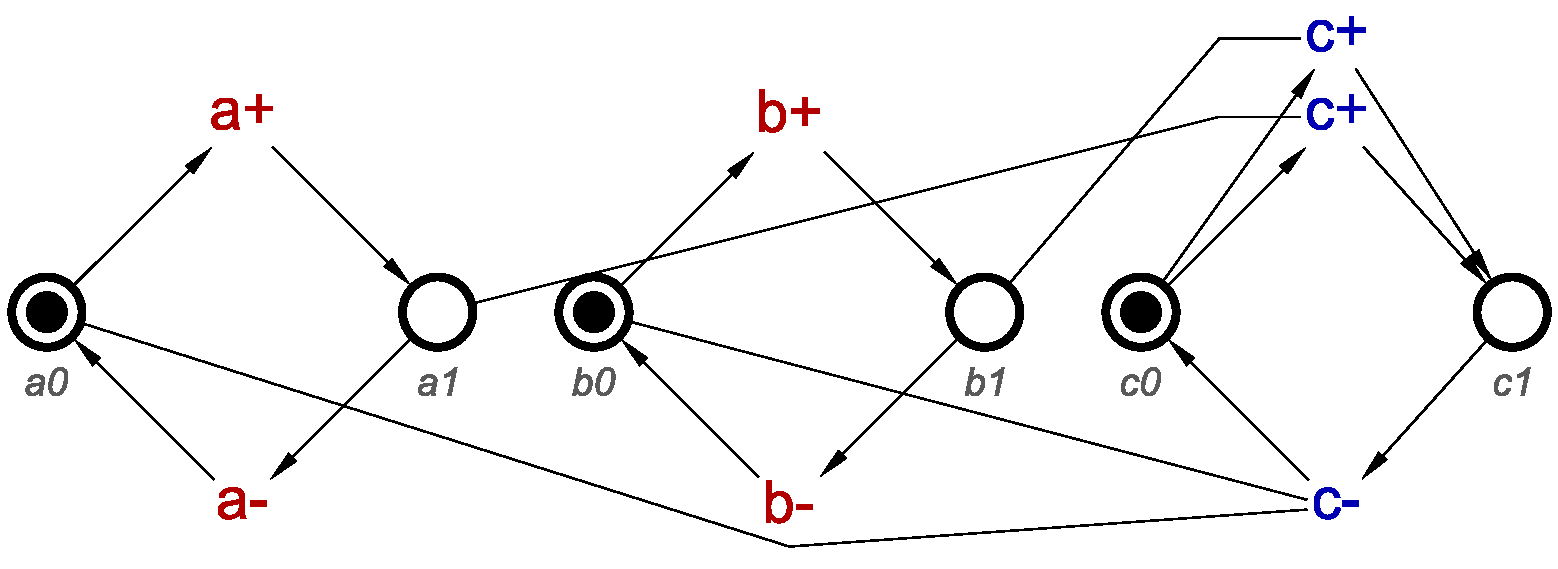
\includegraphics[scale=0.25]{Images/or-gate-stg}
\par\end{centering}
%\vspace{-1mm}
\protect\caption{\label{fig:or-gate-stg} An OR-gate STG}
%\vspace{-3mm}
\end{figure}

This STG features 2 different $c^{+}$ transitions, due to the OR-causality. 
This is for each possible cause, and it is visible that one is connected via a 
read-arc to the $a1$ place and the other is connected via a read-arc to 
the $b1$ place. This allows $c^{+}$ to transition if either $a^{+}$, 
$b^{+}$ or both of these has occured.

Note that there is still only one $c^{-}$ transition, as this requires both
$a^{-}$ and $b{-}$ to have transitioned.

%\vspace{-3mm}

\subsection{AND-gate}

An AND-gate, unlike what the name suggests also features OR-causality. 
For the output to go high, the input signals are in an AND-causality relationship
with the output, however, only one of the inputs needs to transition low for the 
output to go low. 

%\vspace{-3mm}

\begin{figure}[h]
\begin{centering}
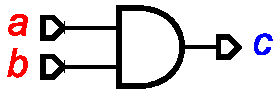
\includegraphics[scale=0.55]{Images/and-gate-circuit}
\par\end{centering}

\protect\caption{\label{fig:or-gate-circuit} The circuit diagram of an AND-gate}
%\vspace{-3mm}
\end{figure}

This example also features 3 signals, $a$ and $b$ which are inputs, and $c$
which is an output:

\begin{itemize}
  \item $a$ - When this signal and $b$ are high, the output should be set high.
  \item $b$ - When this signal and $a$ are high, the output should be set high.
  \item $c$ - This output signal is high when all of the inputs are high, but low when
		\emph{at least} one of the input signals are low.
\end{itemize}

\noindent Again, we can start with the interface: 

%\vspace{-1mm}
\[
\begin{array}{lcl}
\mathsf{interface}&\hspace{-2mm}=&\hspace{-2mm}\mathsf{inputs}[a, b]~\diamond~\mathsf{outputs}[c]
\end{array}
\]

\noindent With the initial state, we can again assume that setting all signals low initially will mean 
that no signals are causing any other signal transitions:

%\vspace{-2mm}
\[
\begin{array}{lcl}
\mathsf{initialState}&\hspace{-2mm}=&\hspace{-2mm}\mathsf{initialise0} [a, b, c]
\end{array}
\]

\noindent Now for signal interactions. For the output to go high, both input signals must
transition high. This concept is: 

%\vspace{-1mm}
\[
\begin{array}{lcl}
\mathsf{outputRise}&\hspace{-2mm}=&\hspace{-2mm}a^{+} \rightsquigarrow c^{+} \diamond\, b^{+} \rightsquigarrow c^{+}
\end{array}
\]

\noindent This concept can also be written as:

\[
\begin{array}{lcl}
\mathsf{outputRise}&\hspace{-2mm}=&\hspace{-2mm}[a^{+}, b^{+}] \sim\hspace{-1.5mm}\&\hspace{-1.5mm}\sim\hspace{-1.5mm}> c^{+} 
\end{array}
\]

\noindent OR-causality is necessary for an AND-gate when specifying the output falling. Either $a^{-}$,
$b^{-}$ or both must occur before $c^{-}$ can occur. In concepts, we list the possible
causes for the effect:

%\vspace{-3mm}
\[
\begin{array}{lcl}
\mathsf{outputFall}&\hspace{-2mm}=&\hspace{-2mm}[a^{-}, b^{-}] \sim\hspace{-1.5mm}|\hspace{-1.5mm}\sim\hspace{-1.5mm}> c^{-} 
\end{array}
\]

\noindent We can now compose these for an AND-gate specification. As with the previous examples
this can be in two forms.

%\vspace{-3mm}
\[
\begin{array}{lcl}
\mathsf{andGate}&\hspace{-2mm}=&\hspace{-2mm}\mathsf{outputRise} \diamond\, \mathsf{outputFall} \diamond\, \mathsf{interface} 
\diamond\, \mathsf{initialState}
\end{array}
\]

\noindent A compact version can be formed in this way:

%\vspace{-2mm}
 \[
\begin{array}{lcl}
\mathsf{andGate}&\hspace{-2mm}=[a^{+}, b^{+}] \sim\hspace{-1.5mm}\&\hspace{-1.5mm}\sim\hspace{-1.5mm}> c^{-} \diamond\, [a^{-}, b^{-}] \sim\hspace{-1.5mm}|\hspace{-1.5mm}\sim\hspace{-1.5mm}> c^{-} \\
&\diamond\, \mathsf{inputs}[a, b] \diamond\, \mathsf{outputs}[c] \diamond\, \mathsf{initialise0} [a, b, c]
\end{array}
\]
\\
\noindent This can now be translated, and the resulting STG can be viewed in Figure~\ref{fig:and-gate-stg}

%\vspace{-3mm}

\begin{figure}[h]
\begin{centering}
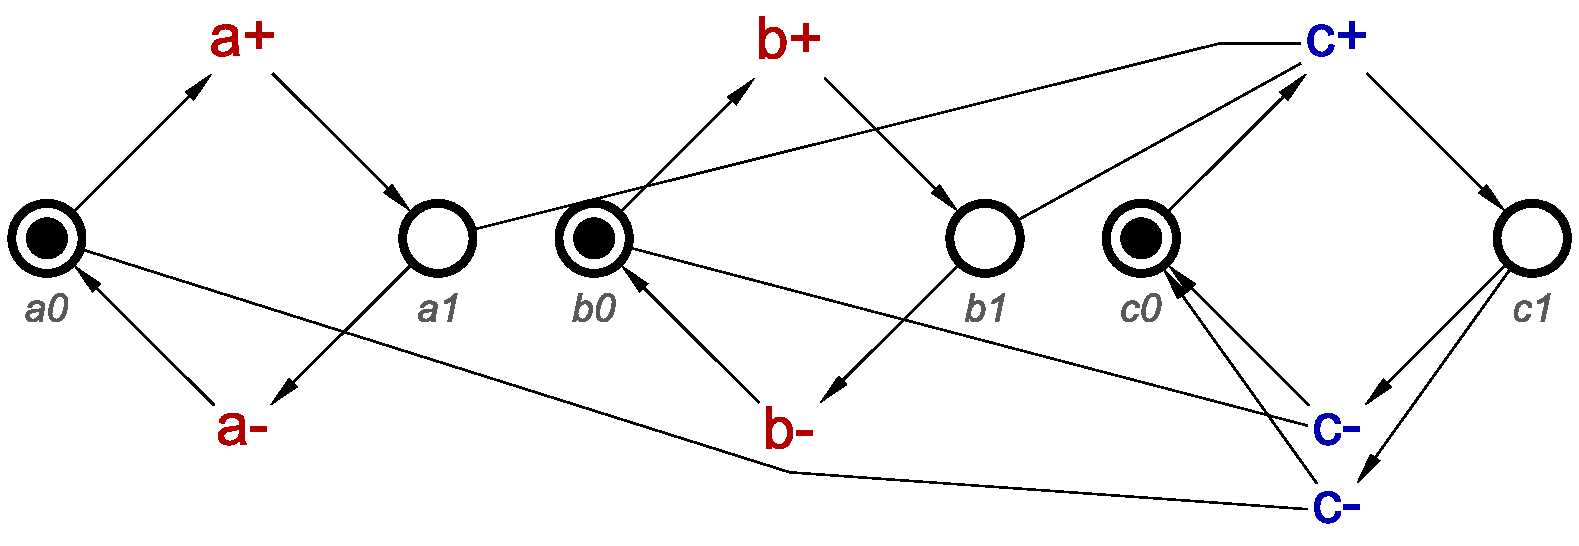
\includegraphics[scale=0.25]{Images/and-gate-stg}
\par\end{centering}
%\vspace{-1mm}
\protect\caption{\label{fig:and-gate-stg} An AND-gate STG}
%\vspace{-2mm}
\end{figure}

This STG is similar to the OR-gate STG~(Figure~\ref{fig:or-gate-stg}), however
in this image, there are two $c^{-}$ transitions, one of which connects to $a0$
via a read-arc, the other of which connects to $b0$. This way, either $a^{+}$ 
, $b^{+}$, or both of these will allow $c^{+}$ to occur. However, both $a$ and
$b$ transitioning high is necessary for $c$ to transition high. 

We have shown the difference that OR-casuality can make to an STG in this
section, but not how this affects the translation. In Section~\ref{sec:algorithm} we 
will discuss the implemented translation algorithm. 

%\vspace{-3mm}
\section{Concepts to STG translation algorithm\label{sec:algorithm}}

Concepts are a useful way of specifying asynchronous circuits, but
specifications also need to be \emph{verified} against certain properties to
ensure their correctness, and once they are deemed to be correct, they need to
be \emph{synthesised} into efficient circuit implementations. Many software
tools exist which automatically verify and synthesise STG specifications,
such as \noun{Petrify}~\cite{Cortadella} and
\noun{Mpsat}~\cite{khomenko2004detecting}.

In order to reuse the tools developed by the community, it is
necessary to be able to automatically translate concept specifications to STGs.
In this section, we will display an example of how the translation algorithm 
operates, and present a pseudocode form of the algorithm in Algorithm~\ref{alg:translation}. 

%\vspace{-3mm}

\subsection{A translation example}

The example we will use for this is that of an OR-gate with control signal. 
This is similar to the OR-gate as seen in Section~\ref{sub:or-gate}; inputs
of $a$ and $b$, and an output of $c$. There will however be an extra 
input signal, $x$. 

This is the control signal, and interacts as follows:
Only when $x$ is high can the output $c$ transition. This control signals
allows a circuit to latch the output signal, by setting $x$ high to let
the output change, and when ready to use this signal, setting $x$ low,
so regardless of the inputs, it will remain in this state, and not change.

This is a rudimentary example, but is useful in displaying how the algorithm
handles a system featuring both OR- and AND-causality. The concept for 
the interaction of the control signal is:

%\vspace{-4mm}
\[
\begin{array}{lcl}
\mathsf{control}&\hspace{-2mm}=&\hspace{-2mm}x^{+} \rightsquigarrow c^{+} \diamond x^{+} \rightsquigarrow c^{-} 
\end{array}
\]

We know this signal is an input, and let's assume we would like to latch
the initially low output signal, and we can include this concept in the 
scenario for this translation:

%\vspace{-3mm}
\[
\begin{array}{lcl}
\hspace{-2mm}\mathsf{orGateCtrl}\,  a \, b \, c \, x &\hspace{-2mm}=&\hspace{-2mm}\mathsf{orGate}\, a\, b\, c \diamond\, \mathsf{control}
\diamond\, \mathsf{inputs}\, [a,\, b,\, x] \\
&& \diamond \, \mathsf{outputs} \,  [c] \diamond\, \mathsf{initialise0}\, [a,\, b,\, c,\, x]
\end{array}
\]

In this concept, we have reused the OR-gate concept, defined in Section~\ref{sub:or-gate}. 
For reference, the fully translated STG can be found in Figure~\ref{fig:or-gate-ctrl}.

%\vspace{-3mm}

\begin{figure}[h]
\begin{centering}
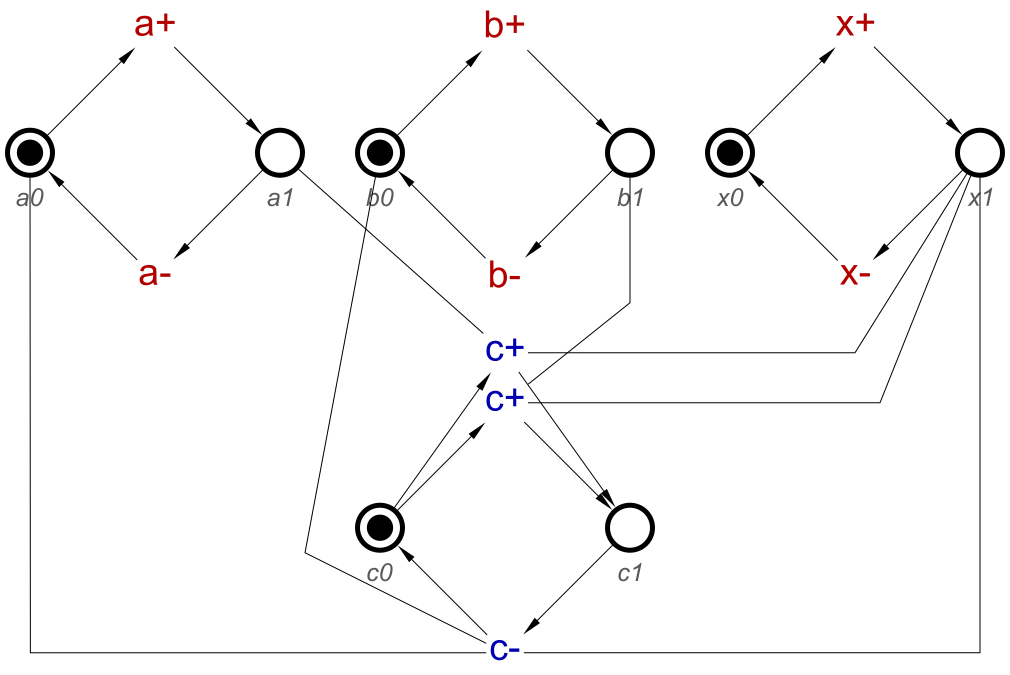
\includegraphics[scale=0.25]{Images/or-gate-ctrl-stg}
\par\end{centering}
%\vspace{-1mm}
\protect\caption{\label{fig:or-gate-ctrl} OR-gate with control signal STG}
%\vspace{-3mm}
\end{figure}

This STG still contains the two $c^{+}$ transitions, allowing this transition when either 
$a^{+}$ or $b^{+}$ has occured. However, with the inclusion of $x$, note that both
of these transitions also require $x^{+}$ to have occured. This is the same for $c^{-}$. 
Through the addition of the \emph{control} concept, we need to add AND-causality to
each and every $c^{+}$ and $c^{-}$ transition with $x^{+}$. The combination of signals
required for each possible transition in both high and low transitions are calculated in the
algorithm, and we will detail this process in this section.

As displayed in Section~\ref{sec:examples}, there are multiple ways of
representing a specification using concepts. However, all levels of
abstraction available to the designer are built out of primitive low-level
signal concepts. Given a specification, we can therefore
break down all gate- and protocol-level constructs into `atoms', which
significantly simplifies the translation task.

For this example, the specification is broken down into these signal-level concepts:

%\vspace{-4mm}
\[
\begin{array}{lcl}
\hspace{-2mm}\mathsf{orGateCtrl}\,a,\,b,\,c\,x&\hspace{-2mm}=&\hspace{-2mm}[a^{+}, b^{+}]\sim\hspace{-1.5mm}|\hspace{-1.5mm}\sim\hspace{-1.5mm}>c^{+} 
\diamond a^{-}\rightsquigarrow c^{-} \diamond b^{-}\rightsquigarrow c^{-}\\
~&\hspace{-2mm}\diamond&\hspace{-2mm}x^{+}\rightsquigarrow c^{+} \diamond
x^{+}\rightsquigarrow c^{-} \diamond \mathsf{inputs} \, [a,\,b,\,x] \\
~&\hspace{-2mm}\diamond&\hspace{-2mm}\mathsf{outputs}\,[c]\diamond\mathsf{initialise0}\,[a,\,b,\,c,\,x]
\end{array}
\]

\noindent The first step is to prepare the read-arcs, and this is done by
reformating these concepts into lists of causes for effects.
Each list will be of possible causes for each OR- and AND-causality signal-level
concept in the specification, meaning that for each OR-causality concept, there will
be 2 or more signals in the list, and for each AND-causality concept there will be a single
item list. 

For example, using the concept $x^{+} \rightsquigarrow c^{+}$, for this $c^{+}$ transition,
there is only one possible cause of it, $x^{+}$. Therefore, this forms a single item list, 
containing only $x^{+}$.

For another example, taking the concept\\$[a^{+}, b^{+}]\sim\hspace{-1.5mm}|\hspace{-1.5mm}\sim\hspace{-1.5mm}>c^{+}$, there are
two possible transitions for $c^{+}$ here, $a^{+}$ and $b^{+}$. These therefore form 
a two item list. 

This will mean there may be several different lists for each cause transition. 
Table~\ref{tab:list-of-concepts} contains all of the lists described above.

\begin{table}[h]
\caption{Lists of possible cause transitions for effect transitions\label{tab:list-of-concepts}}

  \centering
\begin{tabular}[htb]{| m{2.6cm} | m{2.0cm} |}
  \hline
Causes & \, Effect \\ \hline \hline
$x^{+}$ & $c^{+}$ \\ \hline
$a^{+}$, $b^{+}$ & $c^{+}$ \\ \hline
$x^{-}$ & $c^{-}$ \\ \hline
$a^{-}$ & $c^{-}$ \\ \hline
$b^{-}$ & $c^{-}$ \\ \hline
  \end{tabular}
  %\vspace{-3mm}
\end{table}

\noindent From this, we can then combine the lists by effect transition, to give us a list of lists.
This can be viewed in Table~\ref{tab:list-of-lists}

\begin{table}[h]
\caption{Lists of lists of cause transitions for effect transitions\label{tab:list-of-lists}}

  \centering
\begin{tabular}[htb]{| m{2.6cm} | m{2.0cm} |}
  \hline
Causes & \, Effect \\ \hline \hline
[$x^{+}$], [$a^{+}$, $b^{+}$] & $c^{+}$ \\ \hline
[$a^{-}$], [$b^{-}$], [$x^{-}$] & $c^{-}$ \\ \hline

  \end{tabular}
  %\vspace{-1mm}
\end{table}

\noindent Note how for the $c^{-}$ transition there is 3 different single item 
lists. Each one is an AND-causality, and why they are each in a separate list
will become apparent in the next step. 

This step is applying the \emph{Cartesian Product} to each the list of lists
for each effect transition. This will "expand the brackets", combining each
item of each list with every item of every other list, creating a single list which
provides us with the number of this transition and  whicharcs to connect 
for each transition of each type. 
For example, using the list of lists for $c^{+}$:

%\vspace{-3mm}
\[
\begin{array}{lcl}
~&[a^{+}, b^{+}]\, [x^{+}] = [a^{+} x^{+}, b^{+} x^{+}]
\end{array}
\]

\noindent In this example, we combine every item in the first list,
$[a^{+}, b^{+}]$, with every item in the second list, which only 
contains $x^{+}$. This will therefore give us a new 2 item list. 

This list provides us with both the number of $c^{+}$ transitions,
2, and which transitions are the causes of each of these transitions.
The first $c^{+}$ transition will be caused by $a^{+}$ and $x^{+}$,
the second will be caused by $b^{+}$ and $x^{+}$. 

For $c^{-}$, the result of the cartesian product will be a single item,
as combining each item in each list will combine all three of the items 
at once. This will be as follows:

%\vspace{-3mm}
\[
\begin{array}{lcl}
~&[a^{-}], [b^{-}], [x^{-}]  = [a^{-} b^{-} x^{-}]
\end{array}
\]

\noindent There will therefore be only one $c^{-}$ transition, requiring all three
of $a^{-}$, $b^{-}$ and $x^{-}$ to have occured before $c^{-}$
can occur. 

Now, we can list the read-arcs to be connected for each transition of $c$.
This can be viewed in Table~\ref{tab:list-by-transition}.

\begin{table}[h]
\caption{List of all effect transitions and their causes\label{tab:list-by-transition}}

  \centering
\begin{tabular}[htb]{| m{2.6cm} | m{2.0cm} |}
  \hline
Causes & \, Effect \\ \hline \hline
$a^{+}$, $x^{+}$ & $c^{+}(0)$ \\ \hline
$b^{+}$, $x^{+}$ & $c^{+}(1)$ \\ \hline
$a^{-}$, $b^{-}$, $x^{-}$ & $c^{-}$ \\ \hline
  \end{tabular}
  %\vspace{-1mm}
\end{table}

The numbers of the $c^{+}$ transitions are necessary for reference
when definining arcs, for example, $b^{+}$ needs to connect to 
$c^{+}(1)$, not $c^{+}(0)$ or just $c^{+}$ as this can cause 
erroneous arcs to be included. 

For clarity, where there is only one transition, such as with $c^{-}$
we will refer to this simply as $c^{-}$, but this is effectively $c^{-}(0)$.

This concludes the part of the algorithm which defines the arcs
and transitions. Next, the algorithm begins to build the STGs. 

First of all, we need to add places for each signal. These are used to
show whether a signal has transitioned high or low at any point. 
A token in a $0$ place for example shows that that signal has 
transitioned low. We add a $0$ and $1$ place for each signal, 
which for this example gives us $a0$, $a1$, $b0$, $b1$, $x0$, $x1$
$c0$ and $c1$.

The interface is defined at the start of the algorithm, by listing them as $inputs$,
$outputs$ or $internals$, so now we need to include all the transitions, and
connect these to the places to form consistency loops, to ensure that all signals 
in this system can only transition in one way when this signals previous transition
was in the opposite direction. 

This is done by taking each transition, and if it is a $+$ transition, connecting 
the $0$ place for this signal to the transition, then connecting this transition to 
the $1$ place for this signal. Conversely, if it is a $-$ transition, we connect the
$1$ place for this signal to the transition, and connect this transition to the $0$ 
place. Including these will form an STG as shown in Figure~\ref{fig:loops}. Note
that both $c^{+}$ transitions are included in these loops.

\begin{figure}[h]
\begin{centering}
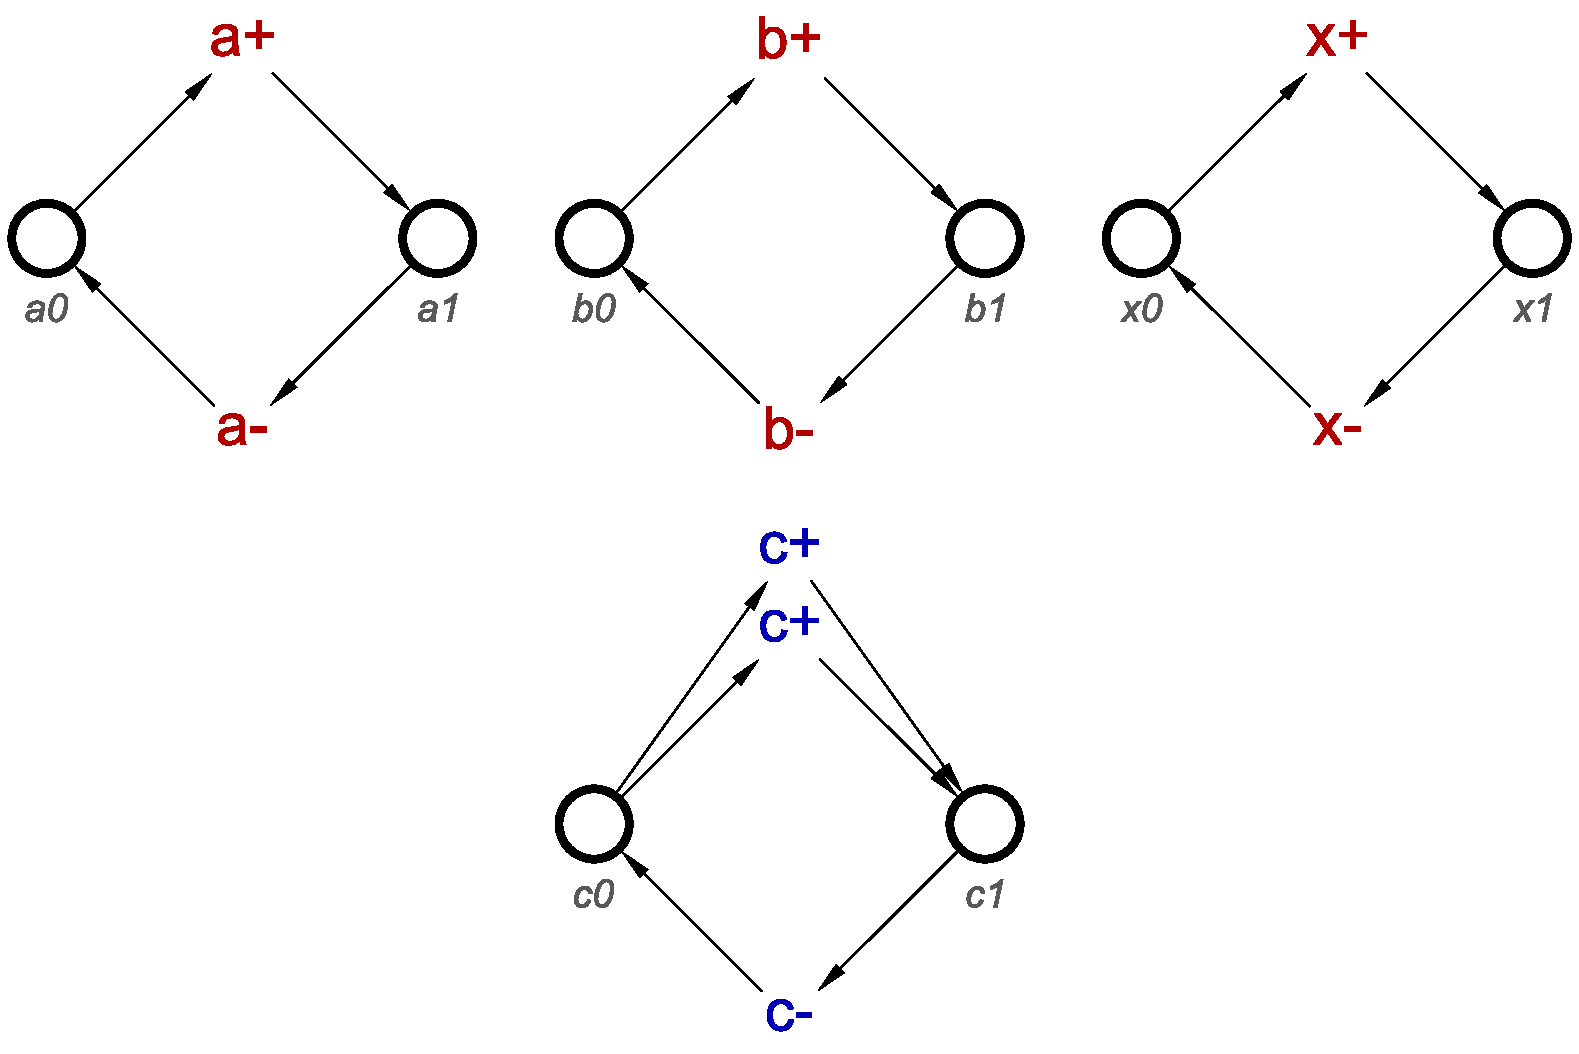
\includegraphics[scale=0.25]{Images/or-gate-ctrl-loops-stg}
\par\end{centering}
%\vspace{-1mm}
\protect\caption{\label{fig:loops} STG containing only consistency loops}
%\vspace{-3mm}
\end{figure}

Now the algorithm introduces the initial states. All of the signals are specified
to be initially 0, meaning that the first transition will be the $+$. From the
consistency loops, to allow this to happen, we need to place a token in each 
$0$ place for each signal. This will produce the STG displayed in Figure~\ref{fig:tokens}.

\begin{figure}[h]
\begin{centering}
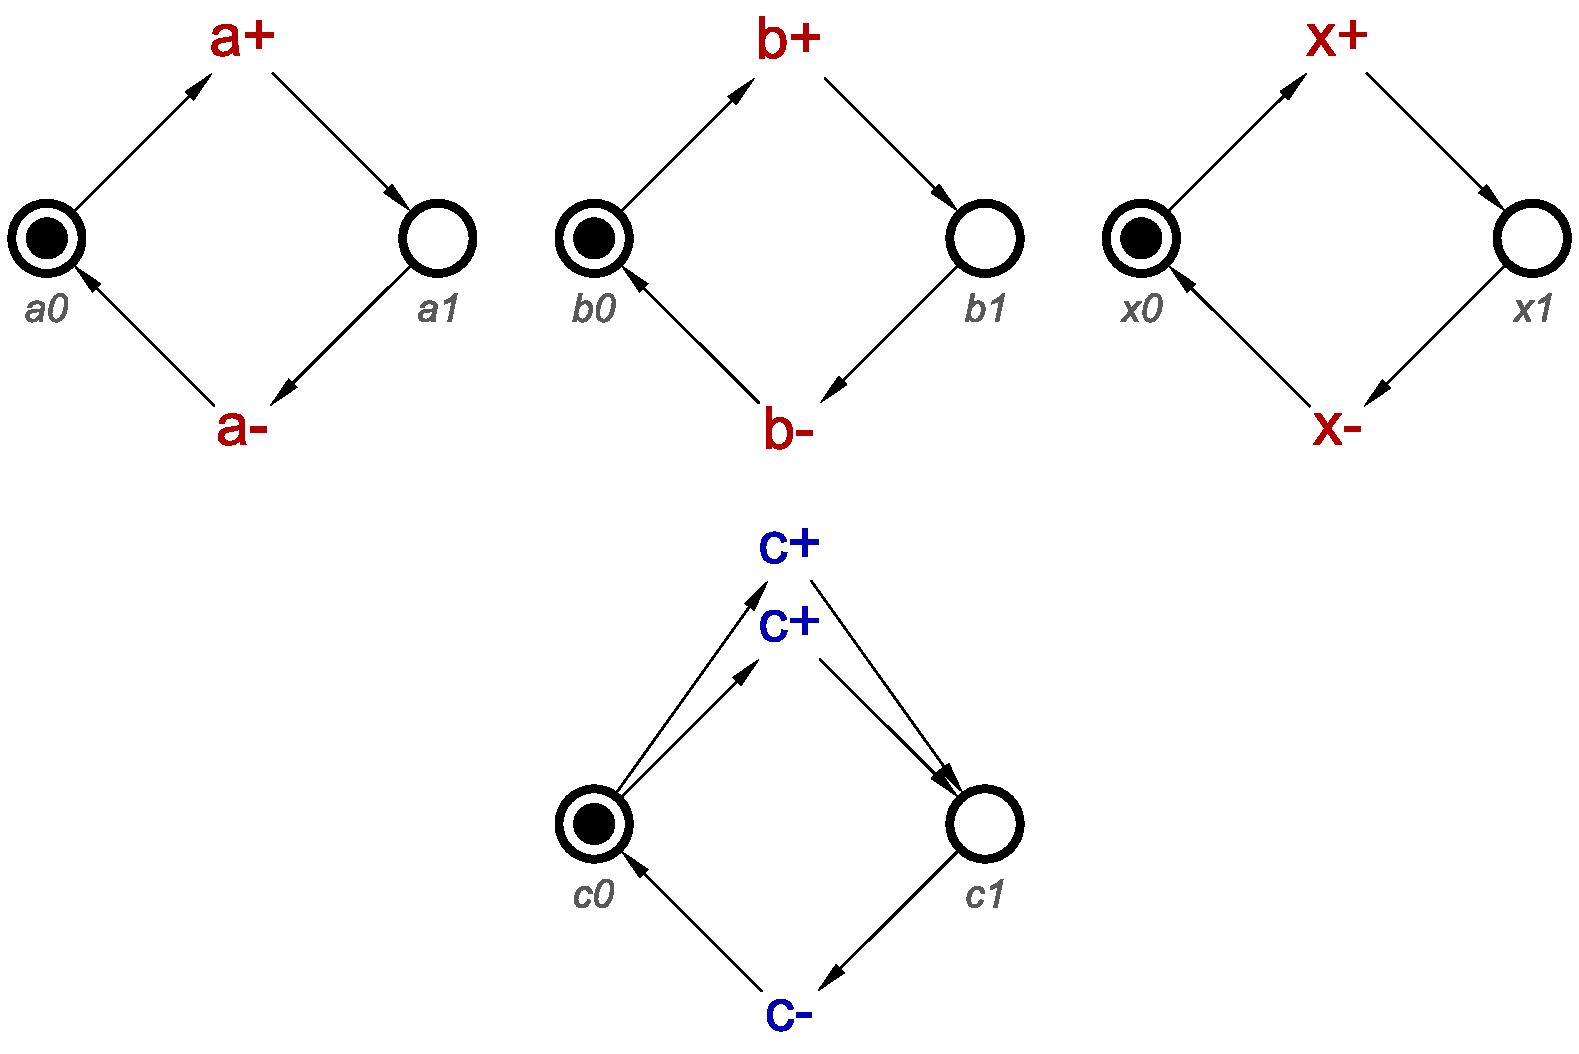
\includegraphics[scale=0.25]{Images/or-gate-ctrl-inits-stg}
\par\end{centering}
%\vspace{-1mm}
\protect\caption{\label{fig:tokens} STG containing consistency loops and initial states}
%\vspace{-3mm}
\end{figure}

Finally, we can add the connections to the transitions, and cause the 
expected interaction between signals. We use read-arcs to connect the effect
transitions to the places after the transition of the cause. For example, for
$x^{+} \rightsquigarrow c^{+}$, we will connect the $x1$ place to the 
transition of $c^{+}$. We use read-arcs for these, as for this example, only
after $c^{+}$ has occured, and placed a token in $x1$, will $c^{+}$ be allowed
to occur, but the read arc will not consume the token in $x1$ which would block
$x^{-}$ from being able to occur. 

Following this, the specification is fully translated, and the resulting STG will
be the same as shown in Figure~\ref{fig:or-gate-ctrl}.


%\vspace{-1mm}

\begin{algorithm}[H]
\begin{algorithmic}
\caption{Algorithm for translating concepts to STGs\label{alg:translation}}
\For {Signal $s$ in \textbf{System}}
  \State \textbf{define} interface of $s$ as \emph{Input/Output/Internal}
\EndFor

\For {Each effect transition $e$}
  \State $allCauses$ $\leftarrow$ Concatinate lists of possible causes for $e$
  \State $transitionList$ $\leftarrow$ \emph{Cartesian Product} \textbf{of} $allCauses$
  \For {$i = 0$ to Length of $transitionList$}
    \State \textbf{add} $e(i)$ to $transitions$
  \EndFor 
\EndFor
\For {Each \textbf{signal} $s$ in system}
  \State \textbf{add} place \textbf{$s$.Name}$0$
  \State \textbf{add} place \textbf{$s$.Name}$1$
\EndFor
\For {Each \textbf{transition} $t$ in $transitions$}
  \If {transition is high}
    \State \textbf{connect} (place $t$.signalName$0$, transition)
    \State \textbf{connect} (transition, place $t$.signalName$1$)
    \For {Each \textbf{cause transition} $c$ for $t$}
      \State \textbf{read-arc} (place $t$.signalName$1$, $c$)
    \EndFor
  \EndIf
  \If {transition is low}
    \State \textbf{connect} (place $t$.signalName$1$, transition)
    \State \textbf{connect} (transition, place $t$.signalName$0$)
    \For {Each \textbf{cause transition} $c$ for $t$}
      \State \textbf{read-arc} (place $t$.signalName$0$, $c$)
    \EndFor
  \EndIf
\EndFor
\For {Each initial state $state$ concept}
  \If {$state$ is low}
    \State \textbf{add-token}(\textbf{signalName.place}$0$)
  \EndIf 
  \If {$state$ is high}
    \State \textbf{add-token}(\textbf{signalName.place}$1$)
  \EndIf
\EndFor
\end{algorithmic}
\end{algorithm}

%\vspace{-2mm}

\subsection{Interoperability with STG based tools \label{sub:interop-with-stg}}

The concepts tool, which translates asynchronous concepts to STGs has been
integrated into open-source toolsuite \noun{Workcraft}~\cite{Workcraft_website}.
This allows a designer to visualise their concept designs as STGs, to simulate,
verify and synthesise them using other tools integrated in \noun{Workcraft},
such as \noun{Petrify}~\cite{Cortadella} and
\noun{Mpsat}~\cite{khomenko2004detecting}.
If there are any corrections or additions to be made these can be done
either directly in the STG or in the original concept specification, which can then
be re-translated into an updated STG. These automated processes can allow for a
streamlined design process of asynchronous circuits.

The translation tool itself produces a \emph{.g} document format, which is a
graph format used to store STG information. This means that it is not
necessary to view the STG after translation, and a concept specification
can be used directly after translation with these tools. 

%\vspace{-3mm}

\section{Conclusions and future work\label{sec:conclusions}}

In this work we show that it is possible to design asynchronous control
circuits at the interface between analogue and digital worlds by
splitting their specification into operational modes, scenarios, and
describing signal interactions and requirements of each scenario using
high-level asynchronous concepts. These can then be translated into STGs
that represent these operational modes, which can be used with existing
verification and synthesis tools. STGs can be further combined to
produce a complete model for the system specification.

In this work, we show some more possibilites available when desingning
asynchronous control circuits using concepts. OR-causality can be a
useful tool to include in a circuit, and providing a seemless method
of translation of both this, and the more common AND-causality allows
for concepts to be used in the design of a wider range of asynchronous 
circuits.

Using concepts, a user can reduce the time of designing an asynchronous
control circuit from the ground up, as well as allow reuse of components
either as part of a scenario or entire scenarios to reduce the design-time
of future projects. Composition of concepts and scenarios can help
reduce errors and save time in comparison to performing these manually.
This method can help to make asynchronous circuits more appealing
to industrial designers.

Currently, this method works with Signal Transition Graphs, however
it can be applied to other modelling disciplines, such as Finite State
Machines~(FSM).

\emph{Process mining} can also be used for various purposes in conjunction
with designing asynchronous circuits. For example, process mining can discover
a behavioural model when none currently exists, and can be used to check 
that an existing specification is realistic, or find less complex models. 
All of this can be performed automatically, by tools such as
\noun{PGminer}~\cite{mokhov2016mining}, given
an event log with observations of a real analogue or digital system, and aid a
designer in reducing design time and errors. We aim to test the possibility of producing
concepts directly from the mining of these event logs.

The translations tool we have discussed is available from~\cite{2016_concepts_github},
and as stated, is integrated into \noun{Workcraft}~\cite{Workcraft_website}. 
A manual is included with the tool, which features descriptions of the features. 
We host a regularly updated blog which discusses some interesting properties
of concepts, and new ideas we find for concepts, and this is available 
at~\cite{2016_blog_concepts}.

%%\vspace{-2mm}

\bibliographystyle{unsrt}
\bibliography{publications}

\end{document}
